\chapter{Quantum (Anomalous) Hall Effect Circulators}
\label{sec:hall}

While discussing architectural concerns in Chapter~\ref{sec:arch}, we focused a great deal on the need to reduce the complexity of interconnects,
particularly as 2D architectures are scaled up. In doing so, we discussed the need for attenuation in the control wiring of a quantum computer
to reduce the thermal population of photons at the qubit interface. Similarly, there is a need for isolation in the readout chain, however
as we explored in Sec.~\ref{sec:readout}, the effective noise temperature $T_\textrm{eff}$ is set by the first stage amplifier and by any attenuation
which occurs between it and the qubit. As such, particularly for transmon-type experiments where any noise is known to limit qubit
lifetimes~\cite{PhysRevLett.101.080502}, passive circulators with low loss must be used. These are non-reciprocal devices which route power
in a single direction around their ports, i.e. from ports $1 \to 2$, $2 \to 3$ and $3 \to 1$, but not in the inverse direction $1 \not\to 3$, $3 \not\to 2$
and $2 \not\to 1$. Furthermore, when using quantum limited parametric amplifiers such as the traveling-wave parametric amplifier~\cite{PhysRevLett.113.157001},
isolators are necessary to limit the action of the pump tone on our qubits. An example of such a circuit is given in Fig.~\ref{fig:circfig} (a), showing
four circulators used for signal routing and isolation.

\begin{figure}[tb]
    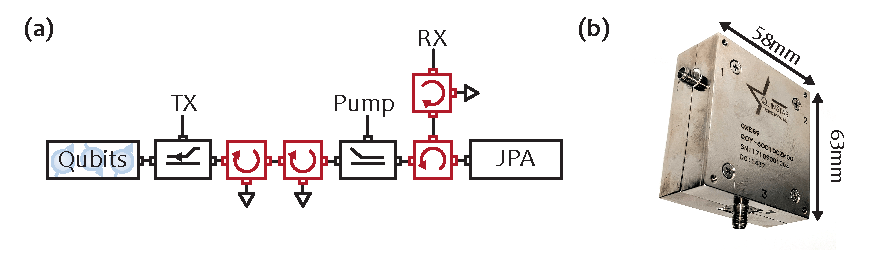
\includegraphics[width=\linewidth]{circ_fig}
    \caption[Schematic of a standard transmon-like experiment]
    {\label{fig:circfig}(a)Schematic of a standard transmon-like experiment. Circulators, outlined in red, are used to provide isolation between amplifiers and qubits,
    and to route signals in the circuit. (b) A conventional circulator based on the Faraday effect.}
\end{figure}

Circulators have traditionally been constructed using the Faraday effect in magnetic materials. This causes propagation to occur at different phase
velocities in opposite directions through a magnetic material, however, as these devices operate based on the interference of counter-propagating paths,
these devices must be constructed with a size on the order of the wavelength of the signal, often several tens of centimeters. An example of such a device is
shown in Fig.~\ref{fig:circfig} (b). It was proposed by
Giovanni Viola and David DiVincenzo that slow, chiral charge density waves in the quantum Hall regime, called edge magnetoplasmons (EMPs), might be utilized to
construct millimeter-scale circulators~\cite{PhysRevX.4.021019}. In the following chapter, I present work that implements this idea to form non-reciprocal
devices and demonstrate strong isolation (up to \SI{40}{\decibel}). The physics of EMP's is introduced originally in Sec.~\ref{sec:emp}. In Sec.~\ref{sec:hallcirc} the
absorption of EMPs is explored in GaAs, and we use these EMPs to form a micron-scale circulator. In Sec.~\ref{sec:spinhallcirc}, we use the quantum anomalous Hall
effect to create circulators that can operate at zero external magnetic field. The dissipation of power is investigated as a function of temperature and applied signal
amplitude, although the nature of this dissipation remains an open question.

\clearpage
\section{On-chip Microwave Quantum Hall Circulator}
\label{sec:hallcirc}
\import{chap3/}{qhe_circ}

\clearpage
\section{Zero-Field Edge Plasmons in a Magnetic Topological Insulator}
\label{sec:spinhallcirc}
\import{chap3/}{ti_circ}
